\section{Part A: Defining the Application}
\subsection{High-Level Description}
Our goal is to implement a large-scale Elephant Tracking and Monitoring System across the \textbf{Neyyar Wildlife Sanctuary}. This Sanctuary is near cities like \textit{Trivandrum} and \textit{Madurai} and is encircled by many villages. For both the safety of elephants and of residents nearby to this sanctuary, it is crucial to montior the movements of these elephants. The system will consist of a set of \textbf{infrared-equipped} IoT nodes that will detect and beacon out their location based on heat signatures. Infrared will work exceptionally well as it is a \textbf{non-intrusive}, \textbf{non-visible} way to detect elephants. Subsequently, elephants also emit a lot of heat (as an innate property of body heat generated $\propto$ body mass), making it an ideal way to detect elephants.

The size of our deployment will be over several hundred square miles, making range and power efficiency imperative, coupled with the rough and forrested terrain of the sanctuary. 
\begin{figure}[h!]
    \centering
    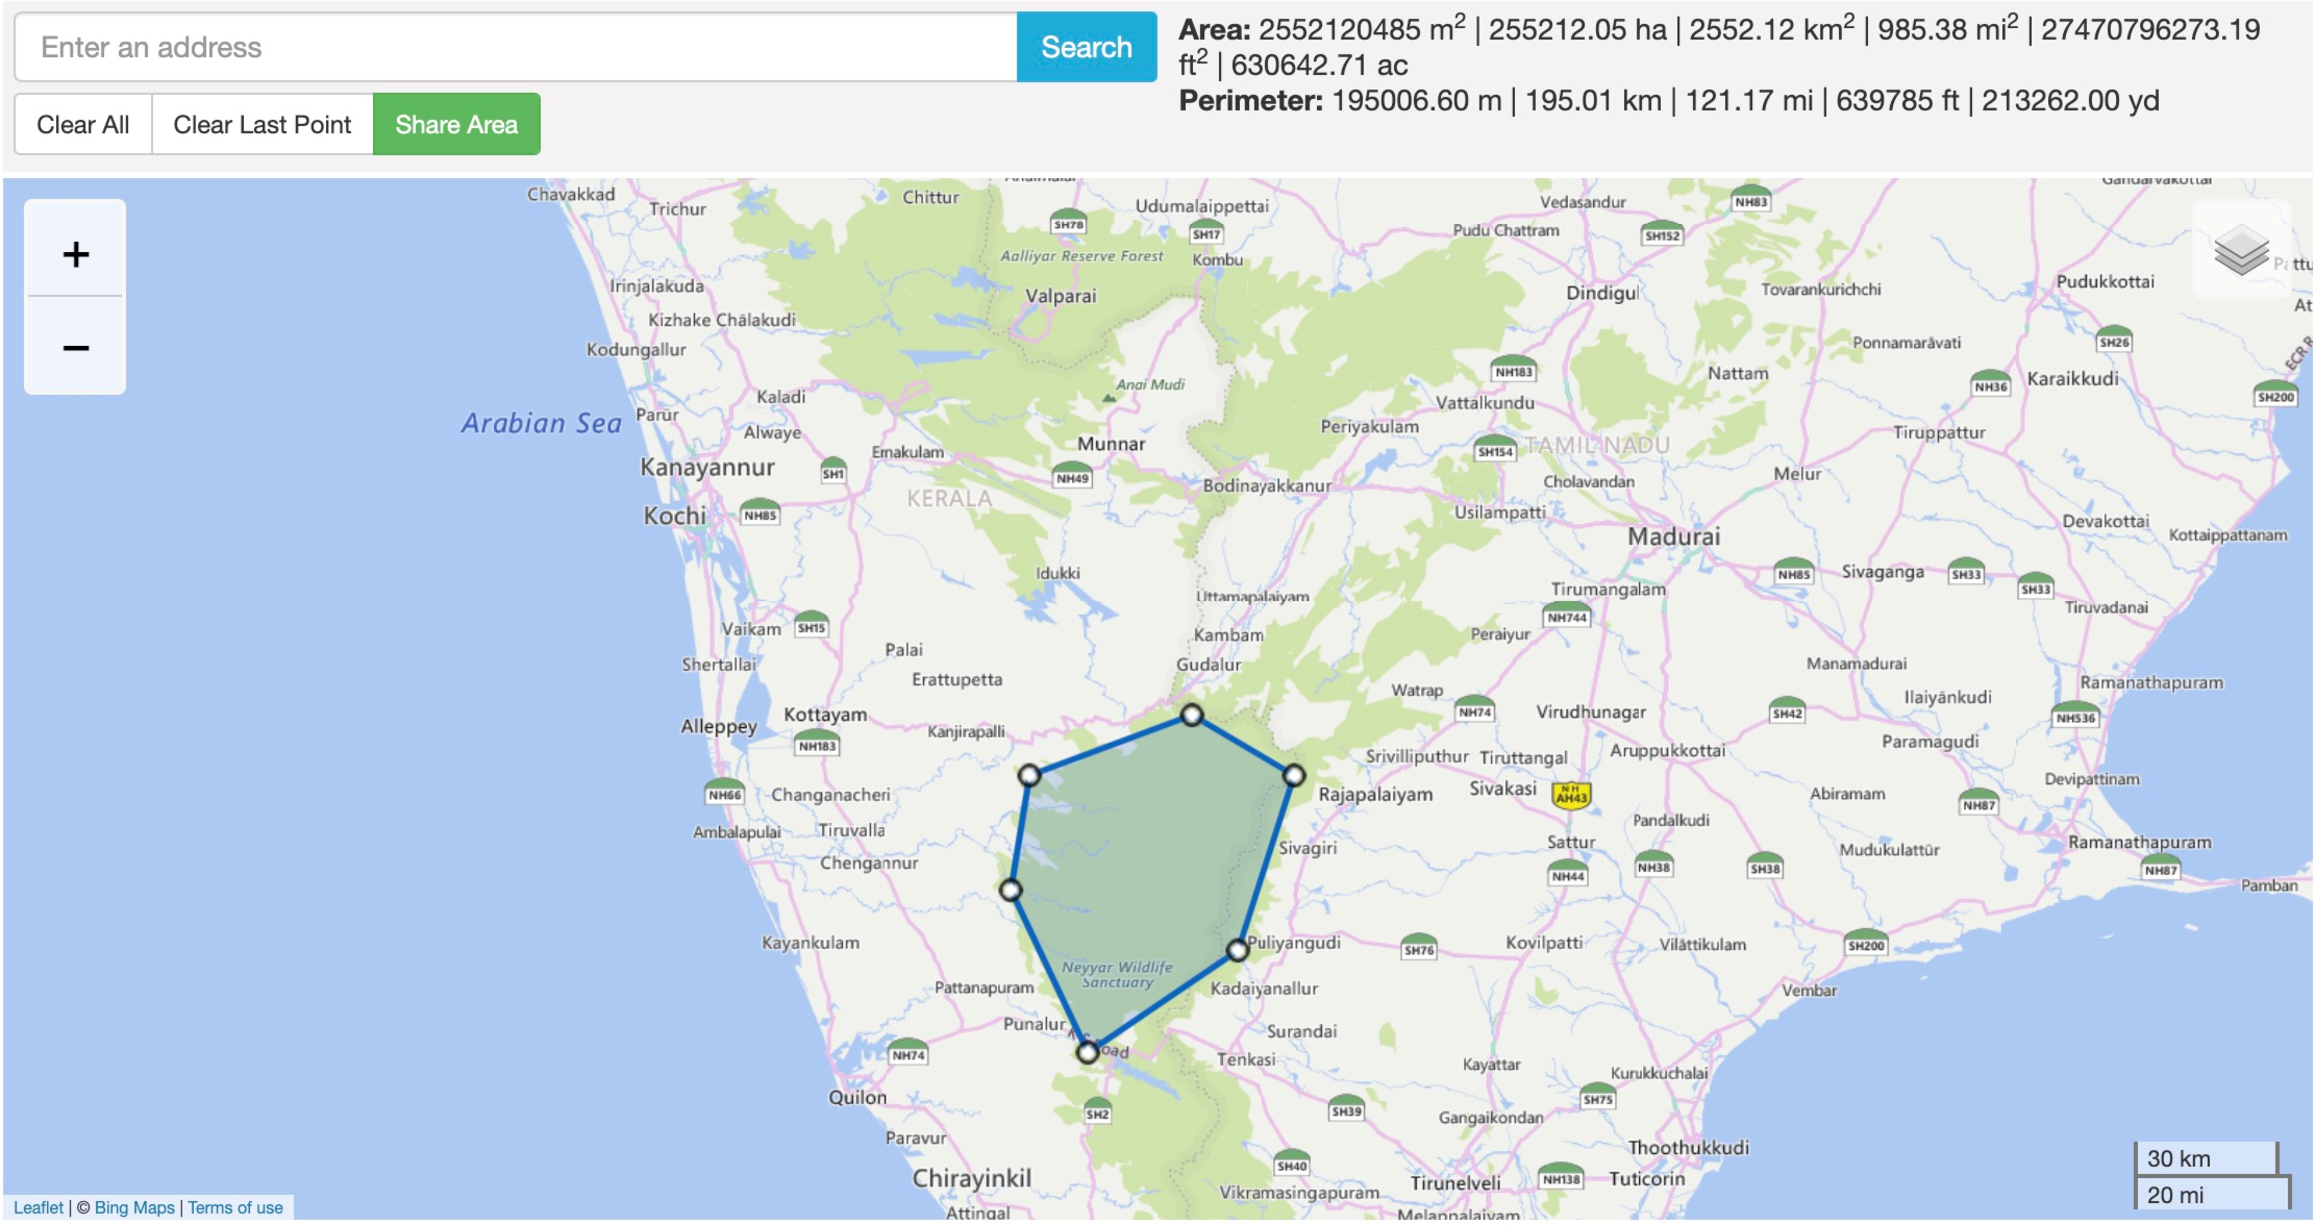
\includegraphics[width=\columnwidth]{figures/NeyyarArea.pdf}
    \caption{Neyyar Wildlife Sanctuary, Kerala, India. Total Area $\approx$ 985 mi$^2$.}
    \label{fig:neyyar}
\end{figure}
There will be three main operating modes for the system: 
\begin{enumerate}
    \item \textit{Steady-State Sensing:} Periodic detection and transmission of location data.
    \item \textit{Event-Driven Update:} Firmware updates and diagnostic data (e.g., when abnormal behavior is detected).
    \item \textit{Emergency Mode:} In the event of an emergency, the system will switch to a high-power mode to ensure that the elephants are tracked and monitored. (i.e. always transmitting location data, sensing etc.)
\end{enumerate}

The role of each of these is similar to what we have seen in our practical applications of IoT devices in Labs. Steady-State Sensing is akin to the Sleepy End Devices that we developed in Lab 3, where we periodically check in with the network and are awoken from sleep should our sensor detect anything or we need to listen from an update from the wider network. Event-Driven Update is akin to the firmware updates that we saw were a necessary condition in Homework 2. Finally, Emergency Mode is just the device will remain on and always transmitting data, in dire situations where an Elephant Habitat is moving towards a village, traffic, or other dangerous areas.

\subsubsection{Steady State Sensing}
In this mode, the nodes will be in a low-power state, waking up periodically to check for elephants. Every 5 minutes, the nodes will simply periodically transmit their location data to a base station. 

Our packet will look like: 
\begin{itemize}
    \item \textbf{Header:} 1 byte
    \item \textbf{Location Data(Latitude, Longitude):} 8 bytes
    \item \textbf{Timestamp:} 4 bytes
    \item \textbf{Elephant Detected/Present}: 1 byte
    \item \textbf{Battery Level:} 1 byte
    \item \textbf{Health Status:} 1 byte
    \item \textbf{Total:} 16 bytes
\end{itemize}

\subsubsection{Event-Driven Update}
In this mode, the nodes will be doing diagnostic work, similar to the firmware updates we saw in Homework 2. Either by clearing out old data, or by checking for any abnormalities in the data that is being collected. Also firmware updates that will be carried out once every month will be done in this mode. (As our application is in a remote area, we cannot afford to have a lot of downtime for the system, so we will have to do firmware updates in a way that does not disrupt the system too much). \textbf{Assumption: } I'll assume that our firmware update will be of a similar scope to the ones we did in Homework 2, so a 10 MB update once a month will be done. 

This means that we do this diagnostic clearing and firmware update once a month, batched, and the other times we are either in Steady State Sensing or Emergency Mode.

\subsubsection{Emergency Mode}
In this mode, the nodes will be in a high-power state, always transmitting data to the base station. This will be done in the event of an emergency, where the elephants are moving towards a village, or a dangerous area. This will be done to ensure that the elephants are tracked and monitored at all times. This means that our sensor is always on, and always transmitting data (i.e we'll set a buffer of 10 seconds, and transmit data every 10 seconds). Rather than doing a periodic check and sleeping, this is more of an \textit{active tracking mode}, where our Infrared Sensor is constantly "pinging the environment", and sending updates on movement of the elephants that are in immediate visibility.

In this mode, the packet structure remains the same to ease the transition between modes, and standardize the data parsing and data transmission efforts. However, the frequency of transmission is increased to every 10 seconds, and the data is always being transmitted. 
\begin{itemize}
    \item \textbf{Header:} 1 byte
    \item \textbf{Location Data(Latitude, Longitude):} 8 bytes
    \item \textbf{Timestamp:} 4 bytes
    \item \textbf{Elephant Detected/Present}: 1 byte
    \item \textbf{Battery Level:} 1 byte
    \item \textbf{Health Status:} 1 byte
    \item \textbf{Total:} 16 bytes
\end{itemize}

\subsection{Data Workload}

Simple dimensional analysis reveals the following data workload for our system. We use the formula
\begin{align*}
    \text{Data Workload} &= \frac{\text{Packet Size}}{\text{Time Interval (s)}} \times \frac{60 \text{ s}}{1 \text{ min}} \\
        &\qquad \times \frac{60 \text{ min}}{1 \text{ hr}} \times \frac{24 \text{ hr}}{1 \text{ day}} \\
        &\qquad \times \frac{30 \text{ days}}{1 \text{ month}}
    \end{align*}
With either $\text{Data Rate} = \frac{16 \text{ Bytes}}{5 \text{ min}}$ for Steady State Sensing, or $\text{Data Rate} = \frac{16 \text{ MB}}{10 s}$ for Event-Driven Update.
\begin{table}[ht!]
    \centering
    \small
    \begin{tabularx}{1.1\columnwidth}{l|X|X|X|X}
    \toprule
    Mode & \multicolumn{2}{X|}{Monthly Workload (MB)} & \multicolumn{2}{X}{Yearly Workload (MB)} \\
    \cmidrule(lr){2-3} \cmidrule(lr){4-5}
     & Downlink & Uplink & Downlink & Uplink \\
    \midrule
    Steady State Sensing & 0.00 & $\sim$0.13 & 0.00 & $\sim$1.58 \\
    Event-Driven Update & 10.00 & Negligible & 120.00 & Negligible \\
    Emergency Mode & 0.00 & $\sim$3.96 & 0.00 & $\sim$47.46 \\
    \bottomrule
    \end{tabularx}
    \caption{\textbf{Downlink and Uplink Data Workload per Mode (MB) - Monthly vs Yearly}}
    \label{tab:data_workload}
\end{table}

Table \ref{tab:data_workload} shows the data workload for each mode, both monthly and yearly. Over our year-long pilot, each node will send roughly 1.58 MB in Steady State Sensing (if it remains in that mode for the entire year), receive 120 MB of downlink data in the form of firmware updates, and send 47.46 MB in Emergency Mode. Since many of our nodes will be in Steady State Sensing for a large part of the year, we can expect our Uplink Data Workload to be much closer to $\sim$1.58 MB (perhaps there might be an aggregated usage of 1 month of Emergency Mode across the year, but this varies on the location of the node and the movement of herds). Roughly, we place an upper bound of $\sim47.46$ MB for the Uplink Data Workload, in the worst case, if a node is proximal to a herd that is constantly moving towards a village or a dangerous area.

\subsubsection{Speed}
The speed of our data transmission is crucial, but the size of our packets are quite small. In Steady-State, we are transmitting 16 bytes every 5 minutes, which is a data rate of 0.0533 bytes per second. In Emergency Mode, we are transmitting 16 bytes every 10 seconds, which is a data rate of 1.6 bytes per second. Any Wireless Technology that we choose should be able to handle these data rates, which are quite small compared to the data rates that we see in our daily lives.

As a lower bound, we define that $> 500 Kbps$ is the minimum data rate that we would need for our system. In the event of an emergency mode, we would need to be able to transmit data at a rate of $> 1.6$ bytes per second. But higher data rates would enable us to send packets faster should we wanted to increase the frequency of our transmissions in a future iteration of our system.

\subsection{Stakeholders}

Organizations and Individuals that would be interested in the data collected by this system include: 
\begin{itemize}
    \item \textbf{Wildlife Conservation Agencies:} Agencies such as \textbf{WildlifeSOS}\cite{wildlifesos} and the \textbf{Asian Elephant Support}\cite{aecp} would be interested in the data collected by this system. They would be interested in the movement of the elephants, and the health status of the elephants.
    \item \textbf{Municipalities and Local Communities}: Local Communities like Kattakada, Neyyattinkara, Ambasamudram, and Kadayan, which are all communities near the Neyyar Wildlife Sanctuary, would be interested in the data collected by this system. This could give insights as to where future elephant habitats could be, preventatively moving them away from villages and traffic, and protecting their constituents.
    \item \textbf{Forest Management Teams:} The Forest Management Teams in the Neyyar Wildlife Sanctuary would be interested in the data collected by this system. This could provide more info on where to do xenosurveillance, and where to place more resources to protect the elephants.
\end{itemize}

\subsection{Scale, Latency, and Reliability}

Based on the aforementioned geographic area covered $\sim1000$ sq.mi ($2600$ sq.km). we would assume a pilot of \textbf{1000 nodes}, with a potential to scale to 50000 nodes for even more granular data. The system should be able to provide near-real-time alerts (e.g., within minutes) in the event of an emergency, this is because due to the nature of our problem (elephants moving towards a village, or a dangerous area), we need to be able to act quickly. Occasional packet loss is acceptable, but overall system robustness is essential $<5\%$ packet loss across the network. This metric is individually applied to each node, but a higher bar for "emergency nodes" that are in Emergency Mode. Emergency Nodes should ideally have $<1\%$ packet loss, as they are the nodes that are in the most critical mode of operation, when elephants are proximal to a village or a dangerous area.

The reason why our pilot is so high is due to the range limitations of Infrared Sensors. PIR Sensors have a range of approximately $7$ meters, but due to the animals that we are observing(elephants), that emit a lot of heat, we can assume that the sensitivity of our sensors will be much higher with respect to elephants versus humans. That being said, \textbf{1000 nodes}, gives each node a coverage area of $2600$ meters per node, or around a 28 meter radius around each node. This is a reasonable coverage area, and we can expect that the elephants will be detected by at least one node in the network, or even a cluster of elephants will be easier to detect.



\subsection{Deployment Constraints}

The Nayyer Wildlife Sanctuary is a remote area, and as such, we have the following constraints on our deployment:
\begin{itemize}
    \item Due to the mountainous and forested terrain of the sanctuary, we cannot rely on wired infrastructure. Our nodes will be battery-powered.
    \item It is difficult to put in larger pieces of infrastructure like towers or access points in the sanctuary, so either we must rely on large scale mesh networking, or we must rely on a technology that has a wide range.
    \item We can use already existing NB-IoT or Cellular Infrastructure based on my findings in Homework 2, but we must be able to have a system that can be maintained with minimal maintenance.
    \item The cost of each node should be in the order of $\$50$, with low recurring operational costs. This is because we are deploying a large number of nodes, and we must be able to do so in a cost-effective manner.
\end{itemize}

\subsubsection{Labor and Maintenance}

Our coverage area is quite wide, for the urposes of this report, we will assume that our technicians have access to an all-terrain vehicle to help them easily traverse the sanctuary (and is a reasonable assumption due to the ecological research initiatives already in place in the sanctuary). We will also assume that our technicians are well-versed in the technology that we are deploying, and can easily troubleshoot any issues that arise.

According to \cite{wxkerela}, the cost of hiring a Wireless Technician is $1913$ rupees ($\$22.25$ according to \ref{conv:Rupee}) per month. The cost to also rent a Jeep to traverse the terrain for the day is $6500$ INR \cite{jeeprent} ($\$77.99$ according to \ref{conv:Rupee}). We will assume that our technicians can cover 25 nodes a day at an 8 hour work schedule, and we will hire 10 technicians to cover the 10000 square mile area. 

This means, that it will take 4 days to deploy the entire network of sensors, as every day, all technicians will put up $\frac{25 \text{ nodes}}{ 1 technician} \times 20 \text{ technicians} = 500$ nodes. This is a reasonable time frame for deployment, and we can expect that the network will be up and running in a month.


The cost of labor and travel for the deployment is $(\frac{22.25}{\text{technician}} \times 20 \text{ technicians} + \frac{77.99}{\text{day}}) \times 20 \text{ days} = (\$522.99) \times 4 \text{ days} = \$2091.96$ for the deployment of the network. This is a reasonable cost for the deployment of the network, and we can expect that the network will be up and running in a month. 

In terms of Maintanence, we will assume that the system will be able to operate for a full calendar year with minimal maintenance. This is a reasonable assumption, as we are deploying a large number of nodes, and we cannot afford to have a lot of downtime for the system. But in a 1 year maintence schedule, we will assume that technicians can \textit{inspect} faster than they can install, so 50 nodes a day can be inspected by a technician. 10 Technicians will take on this effort of inspecting the nodes (just to minimize the impact/workload of exploring a remote area), and this will take 7 days to inspect all the nodes. The cost for this effort is $(\frac{22.25}{\text{technician}} \times 10 \text{ technicians} + \frac{77.99}{\text{day}}) \times 2 \text{ days} = (\$300.49) \times 2 \text{ days} = \$600.98$ for the inspection of the network. This is a reasonable cost for the inspection of the network, and can be done towards the end of our year long pilot. 

In the grand scheme of things, this is not as expensive as what my initial estimates placeed the cost of the network at, but this is partly due in part to the fact that the salary wage for Technicians in India is much lower than in the United States (and is also quite oversaturated with a lot of technicians).


\subsubsection{Additional Constraints}
Weather should have minimal impact on the system. In particular, South India is notorious for having Monsoons and rain, so our system should be able to handle high winds and rain and this should minimally interfere with the communications of our system. Subsequently, under these conditions we can allow for a higher tolerance of packet loss ($< 10\%$) in the event of a monsoon or heavy rain, simply due to the fact that the weather is not conducive to the operation of the system. Also since we are in a forest, we must be able to handle the fact that the trees will absorb a lot of the signal that is being transmitted, which exacerbates the weather conditions.

Subsequently, our system should not use any bright or visual cues to detect the elephants, as this could potentially scare elephants away or cause them to act in a way that is not natural. This is why a constraint on the system is that it must be able to detect elephants using Infrared, as this is a non-intrusive and non-visible way to detect elephants.


